\section{Generalized Fission of Sliding Window Filters}
\label{sec:fission}

This section describes our technique for the fission of sliding window
filters. Our technique for filter fission employs an optimization
termed {\it synchronization removal}.  This transformation is applied
to nodes calculating the identity function in the general graph such
that they can be removed, but their communication patterns remain
embedded in the general graph. A description of synchronization
removal is beyond the scope of this paper, for a complete exposition,
please see~\cite{mgordon-phd}.

The fission transformation applied to $f$ by factor $P$ divides $f$'s
work among $P$ fission products: $f_1...f_P$.  After the
transformation, each $f$ performs $M(S,f) /P$ iterations of $f$'s work
function in the steady-state.  The following preconditions must be met
before it $f$ can be fissed by $P$:
\begin{enumerate}
\item Fission products divide the work of $f$ evenly:
\begin{equation}
M(S,f) \mod P = 0 
\label{eq:mod-fiss}
\end{equation}
\item The items remaining in the input buffer of the original filter
  after initialization must be less than the number of items that will
  be dequeued by each fission product:
\begin{equation}
C(f) < (M(S,f) / P) \cdot o(W, f)
\label{eq:fiss-precond1}
\end{equation}
\end{enumerate}

\noindent As Section~\ref{sec:data-par} describes, both of these
preconditions can be enforced on any filter by increasing the
steady-state of the graph. The details of fission on a filter of the
general stream graph are given in Figure~\ref{fig:general-fission}:
(a) the definition of the original filter $f$, (b) the steps of the
algorithm, and (c) details for steps 1-9.


\begin{figure*}
\centering
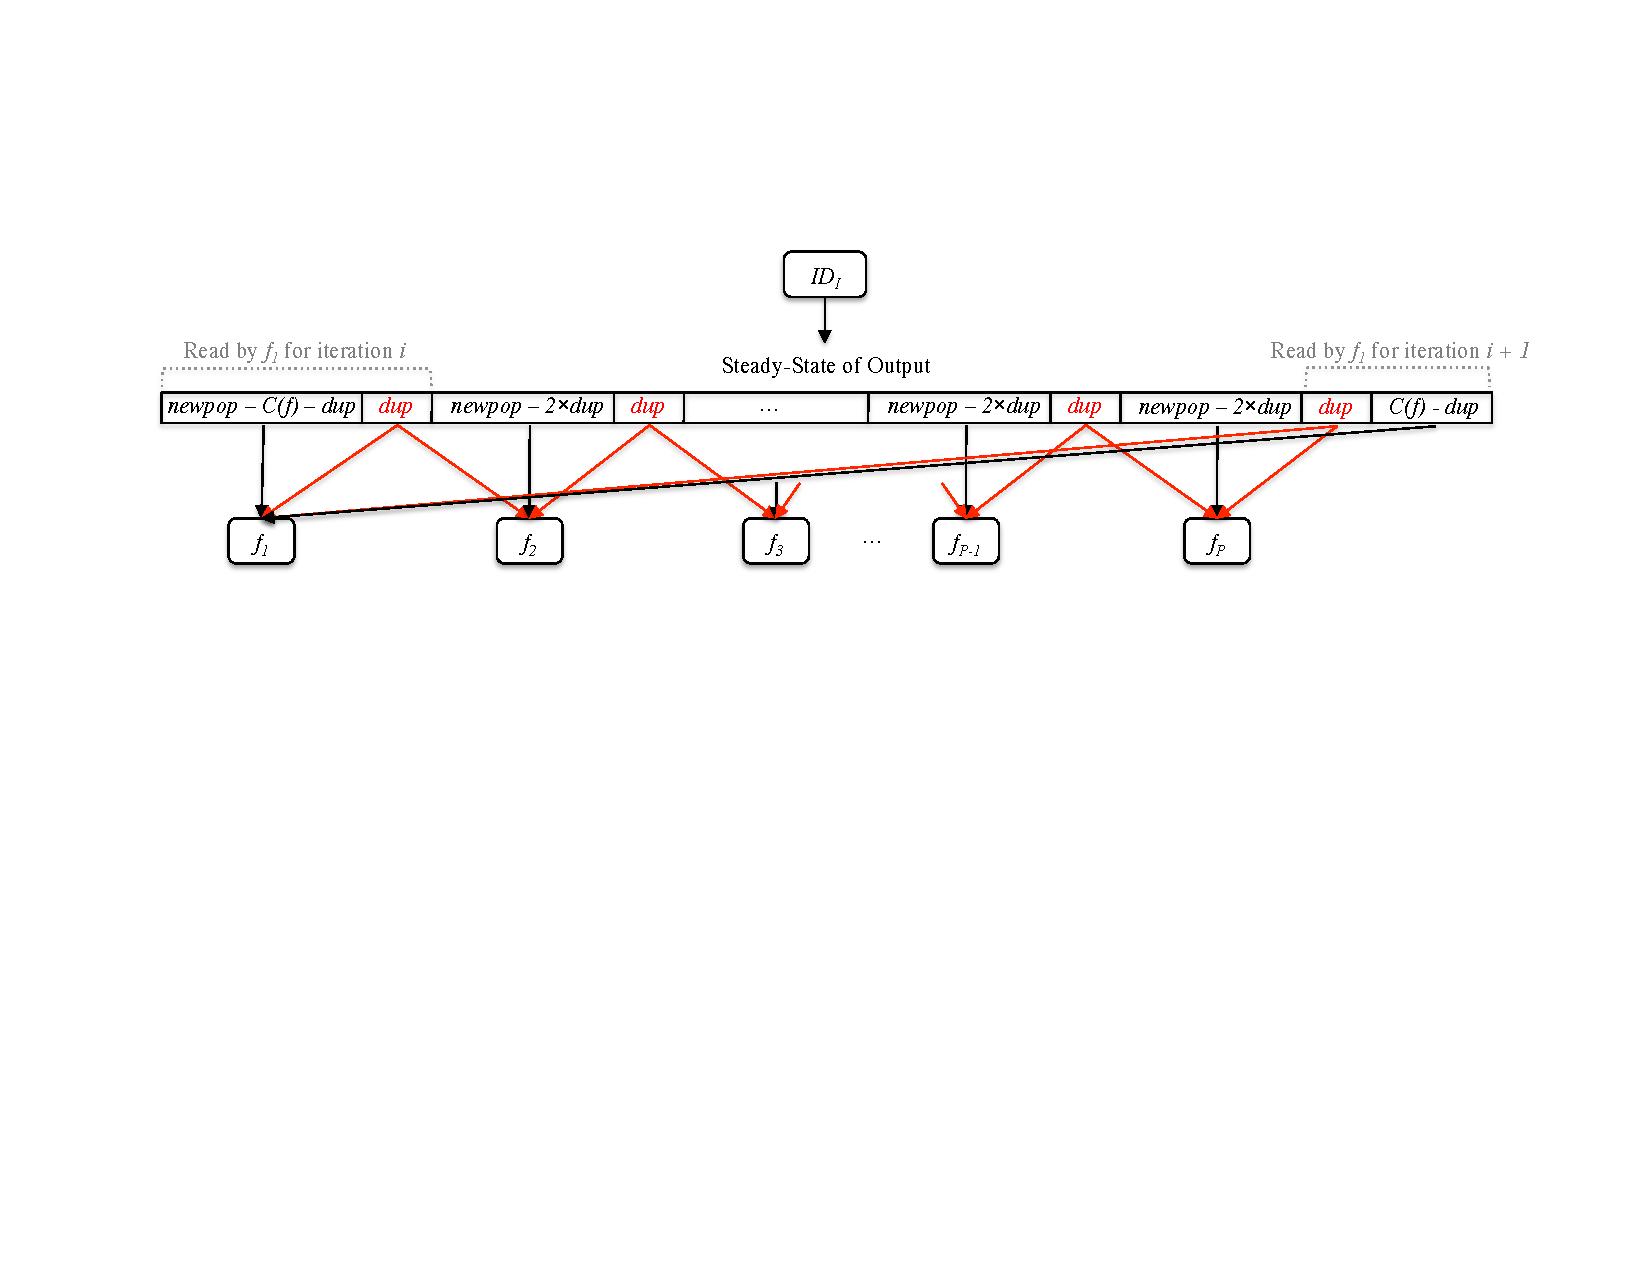
\includegraphics[width=6.3in]{figures/split-pattern.pdf}
\caption[The output distribution required for general
fission.]{
The steady-state output distribution installed for identity node
$ID_I$ by general fission.  Red edges denote items that are shared
across fission products via duplication. If $C(f) > dup$, $C(f) - dup$ items at the end of the
steady-state input are distributed to $f_1$. \label{fig:split-pattern}}
\end{figure*}

The general fission transformation creates two identity nodes ($ID_I$
and $ID_O$) that are encoded to implement the data distribution for
the fission products.  Figure~\ref{fig:split-pattern} illustrates the
pattern of communication between $ID_I$ and the products of $f$.  This
pattern is common to the transformation for all filters we seek to
fiss that meet the preconditions of the transformation.

The fission transformation has the following properties:
\begin{itemize}
\item No item is read by more than 2 fission products.
\item A fission product does not need to remember items across
  steady-state executions of itself. The peeking of the original
  filter $f$ is now encoded in the sharing across fission products
  achieved via the duplication pattern.
\item Only the first fission product $f_1$ is required to receive the $C(f)$
  initialization  items because $C(F) < (M(S,f) / p) \cdot o(W, f)$,
  and it will consume the $C(f)$ items on its first invocation.
\item The presence of the $C(f)$ items in the input buffer after
  initialization must be accounted for by shifting the read pattern
  for the fission products.  The first fission product $f_1$ is offset by
  $C(f)$ items in that it reads its first $C(f)$ items from the
  previous execution stage.  In the steady-state, $f_1$ executing at
  steady-state iteration $i$ shares items with $f_P$ executing at
  steady-state iteration $i-1$.
\item The computation and communication performed by $f$ during the
  initialization stage is transferred completely to the first fission
  product, $f_1$.  Since, by construction, only $f_1$ requires the
  items remaining after the initialization stage.  The other fission
  products are idle during this stage.
\end{itemize}

The final steps of the general fission transformation applies
\textsc{SynchRemove} to remove the identity filters, and stitch the
communication directly between the fission products and $f$'s
producer(s) and consumer(s).
 
%  The process includes the
% following steps (Figure~\ref{fig:general-fission} illustrates steps
% 1-9): 
% \begin{enumerate}
% \item Create $P$ copies of $f$ and set their rates
% and work functions according to Figure~\ref{fig:general-fission}.
% \item Create two identity nodes, $ID_I$ and $ID_O$, that will encode
%   the distribution for the fission.
% \item Move the initialization stage computation of $f$ to $f_1$
%   according to Figure~\ref{fig:general-fission}. 
% \item Move input distribution of $f$ to $ID_I$
% replacing occurrences of $f$ with $ID_I$ in edges.
% \item Move output distribution of $f$ to $ID_O$, replacing
% occurrences of $f$ with $ID_O$ in edges.
% \item Create the fission duplication pattern in the
% output distribution of $ID_I$.
% \item Create a round robin joining pattern for the output identity
%   filter $ID_O$ to receive from each fission product.
% \item For each node $p$ that is a producer of $f$, replace the
%  occurrences of $f$ with $O_I$ in the edges of the dupsets of $p$'s
%  output distribution.
% \item For each node $c$ that is a consumer of $f$, replace the
%  occurrences of $f$ with $O_O$ in incoming edges $c$'s input
%  distribution.
% \item \textsc{SynchRemove}($ID_I$)
% \item \textsc{SynchRemove}($ID_O$)
% \end{enumerate}


% To understand the transformation, we first need to understand the item
% distribution and sharing that is required by fission on a filter $f$
% that adheres to the preconditions above.
% Figure~\ref{fig:fission-sharing2} gives another example of the input
% items required by fission products.  In this example, both:

% \[ C(f) = \mt{dup}_f < (M(S,f) / p) \cdot o(W, f) \]
% \[ M(S, f) \mod P = 0\]

% \noindent so $f$ adheres to the preconditions stipulated above for
% general fission.  In the example, the items read for $f$ plus its
% fission products for $P=4$ are shown for the initialization plus two
% steady-states.  After the initialization stage, $C(f) = 2$ items are
% enqueued to the input buffer by the producer(s) to $f$, and $M(S,f)
% \cdot o(W, f) = 16$ items are enqueued by the producer(s) for each
% steady-state.  Examining the sharing requirement for fission products of
% the second steady-state, we can see a pattern emerge with the following
% features: